\chapter{Inledning}

Energi flödar hela tiden in och ut ur fastigheter, bland annat genom människors aktivitet, ventilation och olika väderparametrar. Dessa energiflöden kan delas in i konstanta och variabla. Vädret är främsta variabla energikällan och vädret kan, genom sina skiftningar, både ge och ta energi från byggnaden. För att bibehålla en jämn inomhustemperatur i fastigheten kan inte en konstant mängd energi tillföras av värmesystemet, utan energitillförseln måste hela tiden regleras efter de opåverkbara energiflödena, där vädret är en stor del.

I dagsläget regleras många fastigheters energisystem endast med avseende på utomhustemperaturen i varje enskilt ögonblick och på så sätt blir det alltid en fördröjning i uppvärmningen. Det leder till ojämn inomhustemperatur och eventuellt också till onödig energiåtgång vilket även gäller fastigheten i det här projektet.

Projektets uppdragsgivare Peter Särneö sköter utrustning för uppvärmning av en äldre fastighet på Walleriusgatan i Göteborg. Han driver ett projekt med syfte att minska energiförbrukningen i fastigheten samtidigt som ett behagligt inomhusklimat bibehålls. Inom ramen för detta har en väderstation och en solintensitetsmätare installerats på taket till fastigheten. Dessa enheter ger en möjlighet att anpassa uppvärmningssystemet till aktuellt  väder. Denna typ av effektivisering av energianvändningen i en fastighet är idag högaktuell på grund av höga energipriser och ökad förståelse för hur vår energianvändning kan påverka klimatet negativt.

% Tidigare kandidatarbeten.
Det har tidigare gjorts tre kandidatarbeten som har undersökt fastigheten på Walleriusgatan. Detta projekt bygger primärt på de två senare, då det första arbetet studerade fastighetens energisystem, vilket ligger utanför ramarna för denna studie. De andra två gjordes åren 2008 och 2010 och då inom området energieffektivisering av fastigheten på Walleriusgatan. 

Det första kandidatarbetet av dessa två \textit{Energiflödet genom ett hus}\cite{kandidatarbete2008},
behandlade mer allmänt energiflödet genom ett hus och hur väl det stämmer
överens med en simulering som gjordes med ett befintligt beräkningsprogram. Arbetet syftade
till att på ett mer fysikaliskt sätt tolka termerna som används för
energieffektivitet. För att kvantifiera energiflödena utfördes mätningar i
fastigheten. Resultaten verifieras med ett välkänt simuleringsprogram,
IDA Indoor Climate and Energy, och slutsatsen är att simuleringsprogramet fungerar bra.
De konstaterar även att för att mäta på fastigheten så är det många parametrar som
måste bestämmas och de rekommenderar utökade mätningar.
 En ytterligare slutsats är att solinstrålningen bidrar till en stor del av
uppvärmningen, och att man för att utnyttja det skulle kunna koppla ett
regulatorsystem till en väderstation.

Det andra kandidatarbetet, \textit{Optimal energihushållning i en fastighet}\cite{kandidatarbete2010},
går ytterligare ett steg och tar fram underlag för att automatisera och
optimera den befintliga fastighetens värmeförsörjning utifrån
flera väderparametrar, fastighetens specifikationer och de boendes verksamhet. Det har i högre grad samma infallsvinklar som detta arbete, men ur ett mer övergripande perspektiv. En stor del av arbetet använder dessutom de avancerade energimodelleringsverktyg ''Revit Architecture 2010'' och 
''EcoTect Analysis 2010'' där en 3D-modell av fastigheten används och även studerar vädrets effekt med en väderfil över Göteborg.

Sedan de tidigare projekten avslutades har fastighetens energiförsörjningssytem uppdateras och detta arbete blir en vidareutveckling av de modeller som kan användas för att modellera hur värme flödar in i och ut ur byggnaden. Vi upplever att det inte är helt utrett hur stor påverkan de olika väderaspekterna, såsom vind, sol och regn, har. Detta är essentiellt för att förstå var de energibesparande åtgärdena ska sättas in för att bli så effektiva som möjligt och för att i förlängningen eventuellt ska kunna dimensionera ett specialanpassat reglersystem.

Ett närliggande område är prognosstyrning av fastigheters energisystem som har både likheter och olikheter med reglering utifrån det momentana och gångna vädret. Båda systemen styr värmesystem i byggnader med hjälp av olika väderparametrar samt byggnadsspecifika parametrar såsom material och täthet. Skillnaden är varifrån den hämtar väderinformationen. Prognosstyrning bygger på prognoser, vilket innebär vissa osäkerheter. När man styr med avseende på det momentana eller gångna vädret är nackdelen att parametrarna redan påverkat inomhustemperaturen innan reglersystemet kan korrigera för dem.

SMHI har under en tid arbetat med prognosstyrning av fastigheter. Deras projekt inleddes med en avhandling inom området av Roger Taesler. Den behandlar främst området ekvivalent temperatur, och från den synvinkeln har SMHI tagit fram ett system som anpassas specifikt till varje fastighet. De har konstruerat ett antal modeller över byggnader där de även tagit hänsyn till byggnadernas läge och när systemet installeras i en fastighet väljs den modell som stämmer bäst överens med det faktiska byggnaden. Systemet tar sedan emot prognoser från SMHI och reglerar radiatorsystemet efter dessa. Systemet är kommersiellt och SMHI förbättrar systemet löpande.

\subsection{Syfte och bakgrund}

\begin{frame}{Bakgrund}

\frame{
  \begin{center}
    \includegraphics[scale=0.7]{../report/images/house.eps}
  \end{center}
}

\section{Dokumentets disposition}

För att göra beräkningar av energiflödena genom fastigheten använder vi oss av några olika beräkningsmodeller. Dessa leder sedan, via våra metoder, fram till resultaten. Nedan finner du en beskrivning av hur.

Efter en inledning med beskrivning av utgångspunkterna för arbetet kommer en del med
 delvis ganska tung teori. Där beskrivs de olika sätt värme kan överföras på – konvektion,
  ledning och strålning – och hur man kan räkna på dem i våra applikationer på 
  energiflödena genom en fastighet. Här beskrivs kort hur de olika delarna av teorin 
  kopplar till våra metoder och resultat. Det är inte alltid nödvändigt för läsaren att 
  tillgodogöra sig all teori för att kunna ta del av resultatet i rapporten. Vi hoppas ändå att 
  det ska kunna visa på att våra resultat står på en gedigen grund.

Strålningen, både från solen och från objekt med avvikande temperatur, av 
svartkroppsstrålning. Vi har speciellt tagit upp när solen skiner in genom ett fönster och då 
modellerat det hela ganska enkelt utifrån solsystemets geometri. På så sätt får vi veta hur 
mycket inomhus luften värms upp vid soligt väder.

För värmeledning och konvektion är den främsta beräkningsmetoden finita 
elementmetoden. För att räkna på konvektionen använder man Navier-Stokes ekvationer 
som modullerar luftflöden. De används även av beräkningsprogrammet Comsol när vi 
modellerar luftflödena i ofrivillig ventilation. Det ekvationssystem som fås ur finita
 elementmetoden optimeras sedan med Newton Raphsons metod.

Dessa olika energiflöden kan sedan beräknas vid olika väderförhållanden. Läggs de 
sedan samman fås en bild av hur mycket energi som måste tillföras fastigheten för att 
bibehålla en konstant inomhustemperatur.

Ett begrepp som sammanfattar energiflödena är free-running temperature som visar på 
vilken temperatur fastigheten skulle ha om man nyttjade den som idag men utan 
uppvärmning. Denna blir givetvis olika för olika väderförhållanden.

I och med vår uppdelning kan vi se var byggnadens störtas energitjuvar sitter och 
olika energibesparande åtgärder kan vägas mot varandra. Om det läcker mest energi ur
 en del av byggnaden är det ofördelaktigt att åtgärda en annan del där det läcker betydligt
  mindre. Vi kan också se vilka väderförhållanden som påverkar energiflödet mest. 
Exempelvis om ett väderförhållande som stjäl mycket energi inträffar relativt sällan tjänar
 man kanske mindre på att åtgärda det än ett som stjäl mindre energi men inträffar väldigt 
 ofta.

Slutligen diskuterar vi var husets största problem, ur energisynpunkt, finns och hur lämpliga olika åtgärder är.

\section{En beskrivning av fastigheten på Walleniusgatan och dess konstruktion}
\label{subsec:thehouse}
% Johanneberg 7:8

% Hur tänkte de när de byggde och renoverade huset?
% Vad ville de uppnå och vilka regler och normer hade man att hålla sig till?

% Att huset är byggt så här vad betyder det för hur huset påverkas och hur huset är att bo i?

% Det är så här stort och har så här många rum, så här högt i tak o.s.v. 

Huset uppfördes 1935\cite{ritningar_urspr} och sedan kom det att dröja ända till 1988 innan den första större ombyggnationen gjordes. Då gjordes två lägenheter om till kontor, stammar byttes och vinden byggdes om till lägenheter. Både taket, burspråken på södersidan och den norra fasaden tilläggsisolerades. I samband med detta installerades också nya värme- och ventialtionssystem och alla fönster tätades med expanderskum. Den främsta skillnaden för de boende blev minskat drag och bättre luftgenomströmmning.  Med det nya venitlationssystemet byts luften helt och hållet varannan timme. Enligt Peter Särneö\cite{petersarneo} förbrukar fastigheten idag mindre energi än ett nybyggt hus.

Fastigheten 13 lägenheter och en kontorslokal på $\unit[225]{m^2}$. De utgör tillsammans $\unit[1450]{m^2}$ fördelat på sju våningar. Utöver detta finns det gemensamma utrymme, trapphus, förråd och apparatrum i den nedre källaren och Peter Särneö\cite{petersarneo} bedömmer att det totalt rör sig om ca $\unit[2000]{m^2}$. Sedan ett tag tillbaka har även en väderstation installerats i förhoppningen att den ska kunna utnyttjas för att förbättra fastighetens klimat ytterligare, se avsnitt \ref{subsec_weathertransmitter}.


% De olika gränsytornas material och uppbyggnad.
\subsection{Väggarna}

Ytterväggarna bestod ursprungligen av 50 cm tegel, klätt med ett centimetertjockt lager av puts på insidan, se figur \ref{fig:sodervagg}. Norrväggen, som tilläggsisolerades i samband med renoveringen 1988, har dessutom 2 cm puts, 10 cm mineralull och ytterligare 2 cm puts utanpå tegelväggen, se figur \ref{fig:norrvagg}.\cite{kandidatarbete2010}\cite{petersarneo}

\begin{figure}[hpbt]
\centering
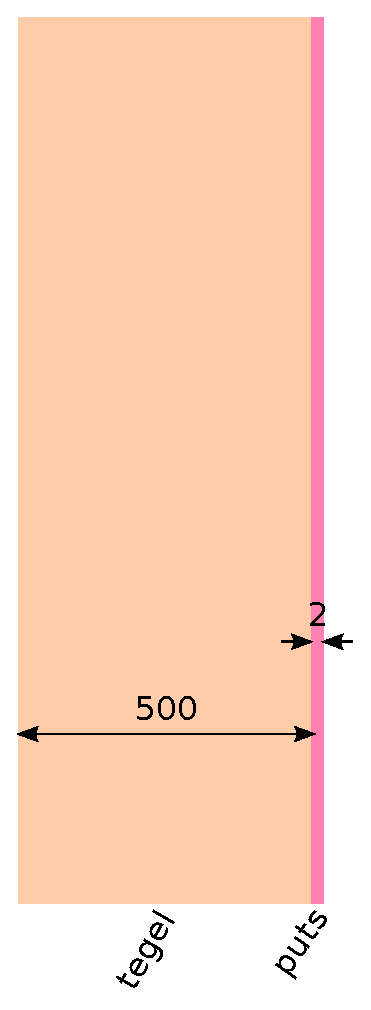
\includegraphics[height=0.3\textheight]{images/sodervagg.eps}
\caption{\label{fig:sodervagg}{Söderväggen, utifrån och in från vänster till höger. Alla mått är i mm.}}
\end{figure}

\begin{figure}[hpbt]
\centering
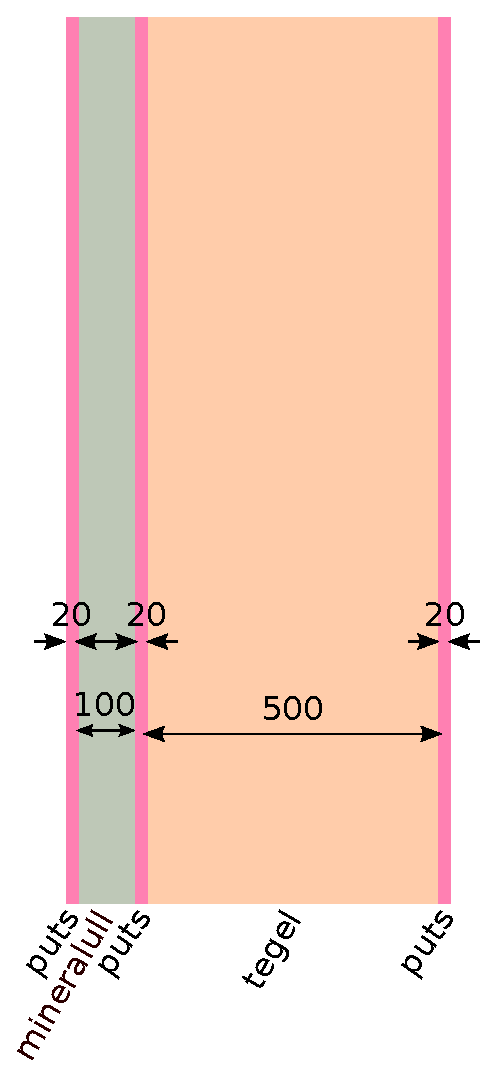
\includegraphics[height=0.3\textheight]{images/norrvagg.eps}
\caption{\label{fig:norrvagg}{Norrväggen, utifrån och in från vänster till höger. Alla mått är i mm.}}
\end{figure}

Fastigheten mellan två andra byggnader i liknande stil. Det öster om är lika högt som fastigheten medan det i väster är något lägre. Fastighetens yttervägg i väster är inte tilläggsisolerad och har samma uppbyggnad som söderväggen, se figur \ref{fig:sodervagg}.

På söderväggen finns ett burspråk som är kopparklätt kopparn sitter direkt på en cementbunden spånskiva och sedan en luftspalt om ca 2,5 cm. Väggen innanför består av 1,6 cm gips, 5 cm minneralull och sedan ytterligare 2,4 cm gips, se figur \ref{fig:bursprak}.\cite{kandidatarbete2010} Enligt Peter Särneö\cite{petersarneo} är det burspråket som läcker mest energi.

\begin{figure}[hpbt]
\centering
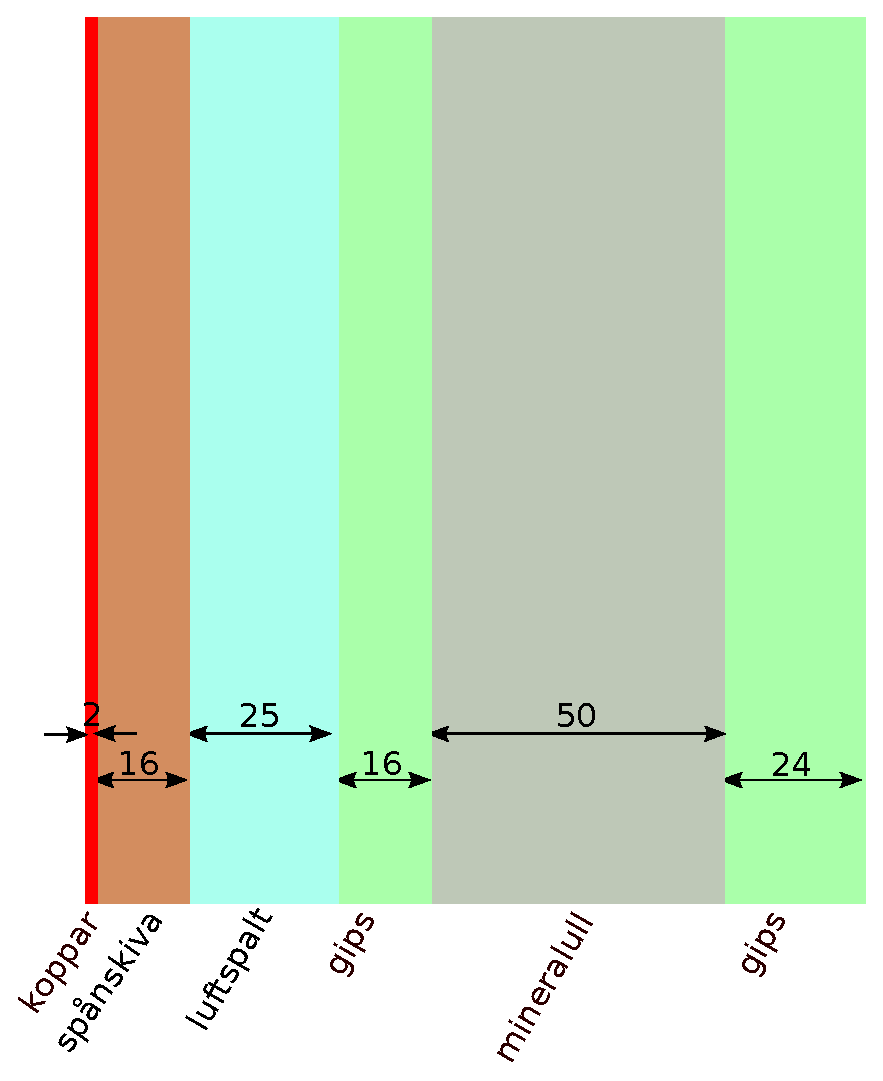
\includegraphics[width=0.3\textheight]{images/bursprak.eps}
\caption{\label{fig:bursprak}{Burspråket på söderväggen, utifrån och in från vänster till höger. Alla mått är i mm.}}
\end{figure}

\subsection{Taket}
Även taket lades om i samband med den stora renoveringen för minskad energiåtgång. Efter det bestod det av taktegel på underlagspapp ytterst, följt av 1,3 cm gips, 21 cm mineralull och innerst ytterligare 2,6 cm gips, se figur \ref{fig:taket}.\cite{kandidatarbete2010}

\begin{figure}[hpbt]
\centering
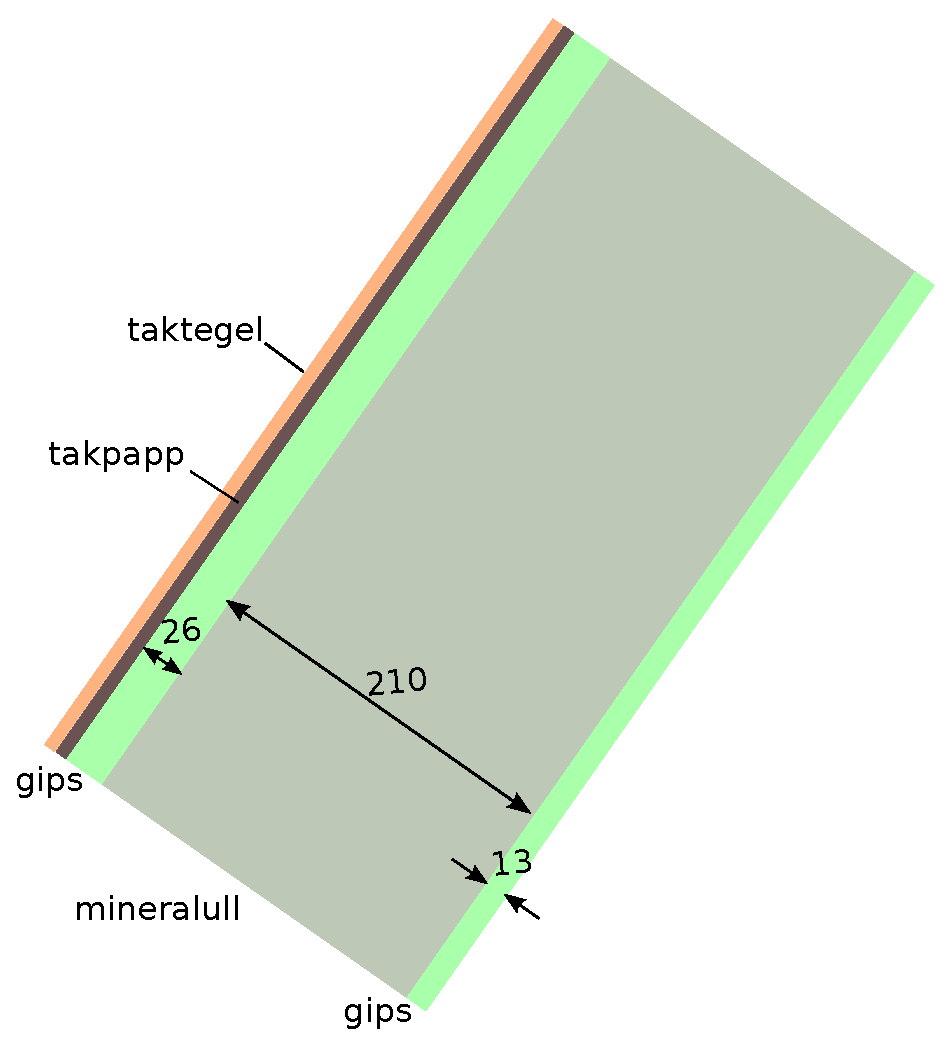
\includegraphics[width=0.3\textheight]{images/taket.eps}
\caption{\label{fig:taket}{Takets uppbyggnad. Alla mått är i mm.}}
\end{figure}

\subsection{Fönstren}

Byggnadens fönster är av treglastyp utan ytbeläggningar. Utrymmet mellan de två innersta glasskivorna är fyllt med argon för att minska värmeledningsförmågan. Totalt får fönstren ett U-värde på ungefär $\unit[1]{W/m^2}$, se avsnitt \ref{sec:heatconduction}. 

\subsection{Grunden}

Huset är byggt på ett berg som sluttar kraftigt. I östra delen av fastigheten ligger huset direkt på berget med endast ett lager av makadam emellan\cite{petersarneo}. I västra halvan har huset en undre källare, det är där apparat- och fläktrummen finns. Där är det betydligt större avstånd ned till berget, uppskattningsvis ett par meter. % Mer exakt? Källa?

\subsection{Uppvärmning och ventilation}
Idag värms huset av bergvärme från tre bergvärmepumpar. För att minska energiåtgången har ett flertal värmeväxlare installerats och värmen från all frånluft återanvänds i möjligaste mån.
% Hur fungerar regleringen? Källa?
Det är viktigt att lägenheterna är kalibrerade så att de får samma temperatur vid samma energiutflöde.

\section{Definition av väder för tillämpningar i denna rapport}
\label{subsec_weather}
Vår uppdragsgivare vill undersöka hur inomhustemperaturen påverkas av vädret. Tesen är att man kan få en mer korrekt styrning av inomhustemperaturen om man inte bara låter den påverkas av utomhustemperaturen, utan även av fler väderparamterar. Han har därför installerat en väderstation, se avnitt~ \ref{subsec_weathertransmitter}.
Begreppet väders vardagliga användningsområde är mycket brett och behöver därför avgränsas för att definiera de väderparameterar som behandlas inom projektet.

Kortfattat definieras vädret som det väderstationen tillsammans med solintensitetsmätaren mäter. Så som finns beskrivet i avsnitt~\ref{subsec_weathertransmitter} mäter vi vädret med utrustning som tar in vindens hastighet och riktning, lufttemperaturen, lufttryck, relativ fuktighet samt regn och hagels varaktighet och intensitet \cite{datasheet_weathertransmitter}. Vi kommer dock att bortse helt ifrån hagel då detta sker så sällan och i så korta perioder att det kan antas försumbart.  Dessutom mäter solintensitetsmätaren solens intensitet och varaktighet, se avsnitt~\ref{subsec:sunmeter}. % Källa på hur ofta (sällan) det haglar i Sverige. 

Tanken är att man ska kunna beskriva allt väder som en temperatur, antingen som den utomhustemperatur man bör reglera efter eller som den inomhustemperatur huset skulle få med befintlig aktivitet men utan uppvärmning, alltså ett mått på hur många grader man måste värma. Dessa två mått kallas ekvivalent temperatur och free-running temperature vilka beskrivs i avsnitt~\ref{sec:ekv_temp} respektive avsnitt~\ref{sec:freerunningtemp}. 

Från studier med hjälp av beräkningstjänsten Wolfram Alpha\cite{wolframalpha} av hur luftfuktighet kan påverkar luftens värmeledningsförmåga, får vi att den har väldigt liten betydelse. Man kan se en liten skillnad vid mycket höga luftfuktigheter (upp emot 90 \%) vid de högre temperaturerna, över $\unit[25]{^\circ C}$. Detta torde vara försumbart eftersom skillnaden är liten och endast vid väderförhållanden som inträffar relativt sällan i vårt klimat.

Hur regn och fukt påverkar fastighetensklimat har inte behandlats inom det här projektet.
Det kan dock antas att en hel del energi försvinner när väggen blir blöt och vattnet avdunstar. Troligen kyler regnet även luften.

Ytterligare en parameter som inte behandlas till är snö. När snön har lagt sig på taket kan man anta att den har en isolerande effekt. Vi kan inte mäta om och i så fall hur mycket snö det ligger på taket. Enligt SMHI\cite{SMHIdata}
rör det sig enbart om 25-50 dygn med snö i Göteborg per år. Detta påverkar dessutom främst de översta lägenheterna, de på vinden. Har man däremot en enplansvilla i Norrland kan man anta att detta är en mer betydande parameter, men det är alltså inget vi kommer att undersöka.

\subsection{Väderstationen}
\label{subsec_weathertransmitter}
I rapporten låter vi de parametrar som väderstationen tar in definiera vädret, se avnitt~\ref{subsec_weather}. Väderstationen som vår uppdragsgivare installerat är en Vaisala Weather Transmitter WXT520. Den mäter sju olika värden: vindens hastighet och riktning, lufttemperaturen, lufttrycket, den relativa fuktigheten samt regn och hagels varaktighet och intensitet. I tabell \ref{tbl:weathertransmitter} beskrivs stationens mätområde, noggrannhet och upplösning för de olika parametrarna. Vi har således väldigt liten nytta av att låta våra beräkningar vara noggrannare än väderstationen kan mäta.

\begin{table}[htdp]
\caption{Tekniska data för väderstationen, \cite{datasheet_weathertransmitter}}

\begin{center}
\begin{tabular}{|l | l l l|}
\hline
\textbf{Väder} & \textbf{Mätområde} % range
 & \textbf{Noggrannhet} % accuracy
 & \textbf{Upplösning} \\ % resolution
\hline
\rule{0pt}{3ex}Vindhastighet & $0$ -- $\unit[60]{m~s^{-1}}$ & $\pm3$ -- $5\%$ & $\unit[0,1]{m~s^{-1}}$ \\ 
\rule{0pt}{3ex}Vindriktning & alla riktningar & $\pm 3^{\circ}$ & $1^{\circ}$ \\
\rule{0pt}{3ex}Temperatur & $-52$ -- $\unit[+60]{^{\circ}C}$ & & $\unit[0,1]{^{\circ}C}$ \\
\rule{0pt}{3ex}Lufttryck & $600$ -- $\unit[1100]{hPa}$ & $0,5$ -- $\unit[1]{hPa}$ & $\unit[0,1]{hPa}$ \\
\rule{0pt}{3ex}Luftfuktighet & $0$ -- $\unit[100]{\%RH}$ & $\pm3$ -- $\unit[ 5]{\%RH}$ & $\unit[0,1]{\%RH}$ \\
\rule{0pt}{3ex}Regn &  & $\unit[5]{\%}$ & \unit[0,01]{mm} \\
~varaktighet & & & $\unit[10]{s}$\\
~intensitet & $\unit[0\mhyphen 200]{mm~h^{-1}}$ & & $\unit[0,1]{mm~h^{-1}}$ \\
\rule{0pt}{3ex}Hagel &  &  & 0,1 $\unit{cm^2}$ \\
~varaktighet & & från första träffen & 10 s\\
~intensitet & & & 0,1 $\unit{cm^{-2}~h^{-1}}$\\
\hline
\end{tabular}
\end{center}
\label{tbl:weathertransmitter}
\end{table}

\subsection{Solintensitetsmätaren}\label{subsec:sunmeter}
Mätaren för solintensitet som finns monterad på fastigheten är en Pyranometer CMP3 av märket Kipp \& Zonen. Den mäter våglängder från $300$ till $\unit[2800]{nm}$, vilket täcker in större delen av den solstrålning som når jorden. Ur databladet fås också att osäkerhet för en dag kan väntas vara under $\unit[10]{\%}$. Den största möjliga instrålningen den klarar av att mäta är $\unit[2000]{W m^{-2}}$ vilket är väl över maximala möjliga värde på jorden om man enbart mäter strålning från solen\cite{physicshandbook}. Den uppfyller gott och väl behoven för studien.\cite{datasheet_sun}





